\subsubsection{Klassifikation af KOLs sværhedsgrad}
Sværhedsgraden af KOL vurderes på baggrund af patienters symptomer, egne erfaringer og livskvalitet. Denne vurderes ud fra Medical Research Council åndenødsskala (MRC) og Chronic obstructive pulmonary disease Assessment Test (CAT). Patienter kan efterfølgende inddeles i klassifikationer med udgangspunkt i MRC og CAT eller ved spirometrimålinger.\cite{Basisbogen2016}

 
MRC-skalaen er en skala fra $1$ til $5$, hvor patienter vurderer mængden af aktivitet, som de kan udføre i forhold til åndenød. Skalaen fremgår af \autoref{tab:MRC}, hvor $1$ svarer til, at patienter først oplever åndenød ved meget anstrengelse, og $5$ svarer til, at patienter oplever åndenød ved meget lav fysisk aktivitet.\cite{Basisbogen2016}

\begin{table} [H]
\centering
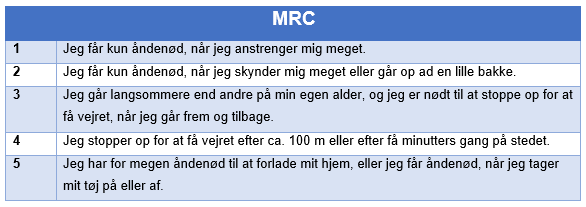
\includegraphics[width=0.9\textwidth]{figures/MRC}
\caption{MRC er en skala fra $1$ til $5$. Patienter, der oplever åndenød ved meget anstrengelse vurderes til $1$, mens patienter, der oplever åndenød ved lav aktivitet vurderes til $5$ på MRC-skalaen. REVIDERET\cite{Basisbogen2016}.}
\label{tab:MRC}
\end{table} 

\noindent
En anden metode til at vurdere symptomerne ved KOL er ved hjælp af CAT-spørgeskema. Her vurderes otte udsagn fra en skala fra $0$ til $5$, hvor ingen symptomer angives $0$. Ud fra de otte udsagn opnås en samlede score, jo højere den samlede score er, desto værre opleves patienters symptomer. Af \autoref{fig:CAT} ses CAT-spørgeskema til vurdering af symptomer.\cite{dsam2016,Basisbogen2016}

\begin{figure} [H]
\centering
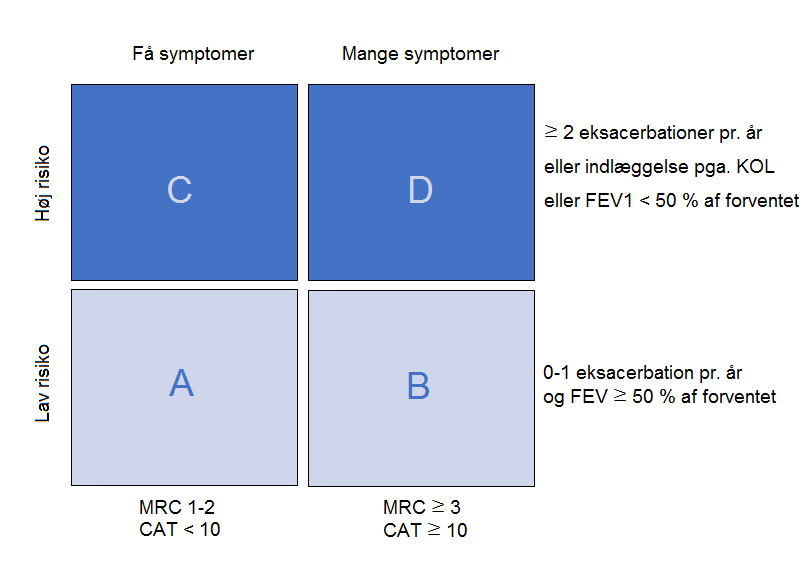
\includegraphics[width=0.5\textwidth]{figures/CAT}
\caption{CAT er et spørgeskema, hvor patienter vurderer graden af deres symptomer ud fra otte udsagn på en skala fra $0$ til $5$. Ingen symptomer svarer til $0$. Patienter opnår en samlede score, jo højere den samlede score er, desto værre opleves patienters symptomer. REVIDERET\cite{Basisbogen2016}.}
\label{fig:CAT}
\end{figure} 

\noindent
Ud fra MRC-skalaen eller CAT-spørgeskemaet samt lungefunktionstest og antallet af eksacerbationer det seneste år kan KOL-patienter kategoriseres. Patienterne kategoriseres i A, B, C eller D, hvor D er patienter i høj risiko og med mange symptomer. Kategoriseringen fremgår af \autoref{fig:KAT}.

\begin{figure} [H]
\centering
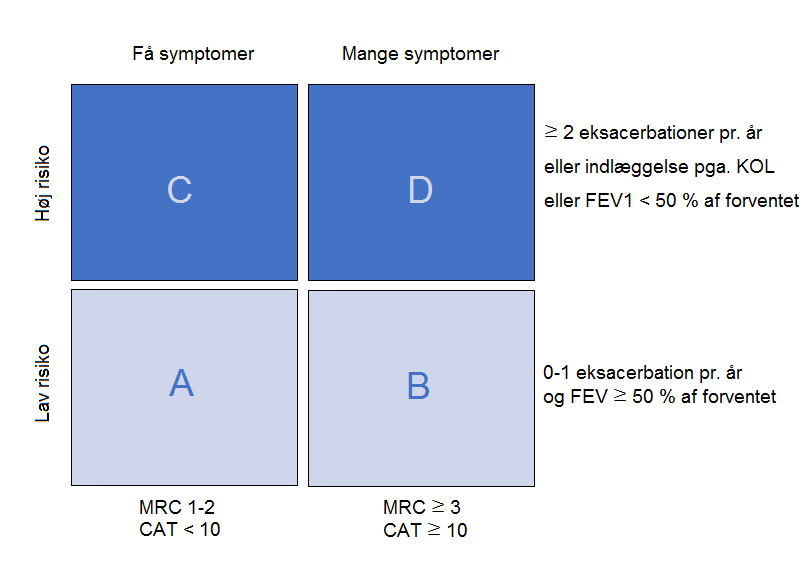
\includegraphics[width=0.8\textwidth]{figures/KAT}
\caption{KOL-patienter kategoriseres i fire kategorier herunder A, B, C og D. A og B inddeles i lav risiko, mens C og D er i høj risiko. REVIDERET\cite{Basisbogen2016}.}
\label{fig:KAT}
\end{figure} 
 
\noindent
Udover ABCD-kategoriseringen kan sværhedsgraden af KOL udelukkende bestemmes ud fra spirometrimålinger.  Sværhedsgraden er klassificeret ud fra retningslinjer opstillet af the Global Initiative for Chronic Obstructive Lung Disease (GOLD).\cite{dsam2016} Lungefunktionen vurderes på baggrund af FEV$1$ i \% af den forventede lungekapacitet, hvoraf det inddeles i fire stadier. Disse fremgår af \autoref{tab:GOLD}.

\begin{table} [H]
\centering
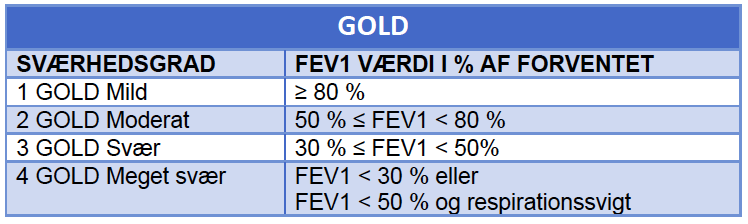
\includegraphics[width=0.8\textwidth]{figures/GOLD}
\caption{GOLD er inddelt efter sværhedsgraderne $1$ til $4$ herunder mild, moderat, svær og meget svær. Patienter, der har over $80~\%$ af forventet lungekapacitet klassificeres som $1$ GOLD mild, mens patienter med under $30~\%$ eller over $50~\%$ af forventet lungekapacitet samt respirationssvigt klassificeres som $4$ GOLD meget svær. REVIDERET\cite{Basisbogen2016}.}
\label{tab:GOLD}
\end{table} 

\subsection{Behandling} \label{sec:behandling}
Det er ikke muligt at helbrede patienter med KOL, da KOL er en kronisk lungesygdom. Dog er det muligt at forhindre udviklingen af KOL samt lindre symptomerne, hvilket kan opnås ved tobaksafvænning, fysisk aktivitet, kostvejledning og medicin.\cite{Basisbogen2016} 

KOL-patienter med sekretproblemer tilbydes continous positive airway pressure (CPAP) eller positive expiratory pressure (PEP-fløjte) og broncodilaterende inhalationsbehandling efter behov og ud fra graden KOL. Yderligere kan antiinflammatorisk behandling gives til patienter med hyppige eksacerbationer.\cite{Basisbogen2016}

Da den tabte lungefunktion ikke kan genvindes, rådes patienterne til ophøre tobaksrygning eller det der kan være årsagen til KOL f.eks. dårligt arbejdsmiljø, hurtigst muligt for således at bibeholde den nuværende lungefunktion \cite{Basisbogen2016}. Det fremgår af \autoref{fig:fletcher}, hvordan tobaksrygning kan påvirke lungefunktionen over tid. 

\begin{figure} [H]
\centering
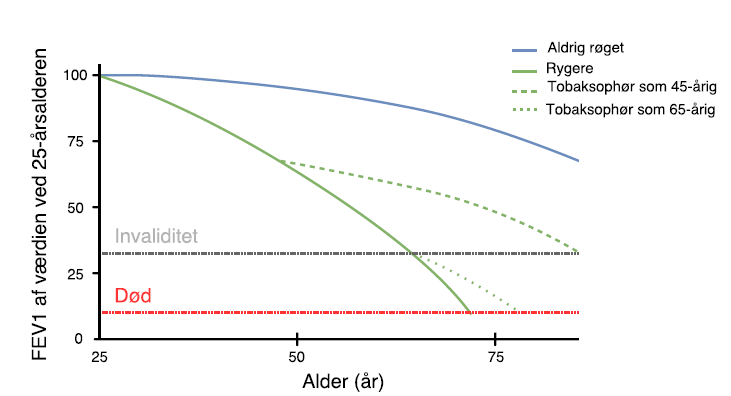
\includegraphics[width=1\textwidth]{figures/fletcher}
\caption{Fletcher-kurve, som viser faldet af FEV1 over tid for henholdsvis rygere, ikke-rygere og rygere med tobaksophør i $45$- og $65$-årsalderen. REVIDERET \cite{Basisbogen2016}.}
\label{fig:fletcher}
\end{figure} 

\noindent
Det ses af \autoref{fig:fletcher}, at tobaksrygning medvirker til et accelererende tab af FEV1, og dermed udsigt til kortere levetid. På trods af tobaksophør genoprettes FEV$1$ ikke, dog bremses det accelerende tab af FEV$1$ til det normale aftag.\cite{dsam2016}

\subsection{Prognose}
KOL-patienter med eksacerbationer har efter indlæggelse en dødelighed på næsten $10$~$\%$ i løbet af den første måned. Dødeligheden ligger på omkring $64$ per $100.000$ per år for mænd og $54$ per $100.000$ per år for kvinder.
Udviklingen, hvormed sygdommen progredierer for KOL-patienter er specielt afhængig af, hvorvidt patienter ophører eksponering til den udløsende faktor for eksempel tobaksophør. Det er derfor vigtigt at få en tidlig diagnosticering således, at patienter hurtigt kan få hjælp.\cite{dsam2016}
%Derudover har et studie vist, at KOL-patienter, der er i stadie $4$ i GOLD-klassificeringen, har lav funktionalitet og livskvalitet, som bliver værre med tiden og ved fremkomst af flere symptomer til sygdommen. \cite{Habraken2011}

